% !TeX spellcheck = es_ES

\title{Adaptaci�n y extensi�n de la herramienta de captura y an�lisis de tr�fico Ksensor\\Dise�o de alto nivel}
\author{Javier Domingo Cansino}

\documentclass[11pt,a4paper]{report} % Para tener un documento grande pero sin ser un libro (solo hay esta posibilidad)
\usepackage[latin1]{inputenc}   % Para la codificaci�n
\usepackage{textcomp}           % Para los simbolos de euro
\usepackage[spanish]{babel}     % Para el lenguaje que tenga bien
\usepackage[T1]{fontenc}        %      los saltos de linea con gui�n etc.
\bibliographystyle{alpha}       % Estilo de bibliograf�a
\usepackage{graphicx}           % Para insertar im�genes
\graphicspath{{../images/}}     % La ruta relativa de las im�genes
\usepackage{hyperref}           % Hacer links guays entre secciones y hacia fuera
\usepackage[hypcap]{caption}    % Hacer que las referencias se vean, y no se queden por encima (referenciando imagenes, etc.)
\hypersetup{
	colorlinks=true,
	linkcolor=blue,
	citecolor=red,
}
\usepackage[table]{xcolor}      % Dar colores a las tablas
\usepackage{eurosym}            % para tener el simbolo del euro
\usepackage{setspace}           % Para hacer el espaciado entre l�neas
\setstretch{1.4}                %      1.4 del espacio normal
\usepackage{parskip}            % El espaciado entre parrafos 
\setlength{\parindent}{25pt}    %      lo ponemos a 25pt
\usepackage[margin=3cm]{geometry} % Cambiar el margen del texto

\usepackage{fancyhdr}           % Cambiar las cabeceras del documento
\pagestyle{fancy}               %      y usar los cambios
\lhead{
\includegraphics[width=5cm]{ingenieros-bilbao}}
\rhead{Adaptaci�n y extensi�n de la herramienta\\ de captura y an�lisis de tr�fico Ksensor}
\cfoot{\thepage}
\setlength{\headheight}{47pt}

\usepackage{titlesec}           % cambiar el estilo soso de los cap�tulos
\titleformat{\chapter}[hang]{\Huge\bfseries}{\thechapter. }{0pt}{\Huge\bfseries}
\usepackage{makeidx}            % Hacer �ndices

% % % % % % % % % % % % % % % % % % % % % % %
% Secci�n de comandos personalizados        %
% % % % % % % % % % % % % % % % % % % % % % %
\newcommand{\reference}[2]{\hyperref[#1]{\textit{\ref*{#1} #2}}}
\makeindex

\begin{document}
\pagenumbering{Roman}
\maketitle % Crear el t�tulo
\tableofcontents % Crear la tabla de contenidos

\pagenumbering{arabic}

% !TeX spellcheck = es_ES
% !TeX root = main.tex
En los últimos años, las tecnologías informáticas de la comunicación están revolucionando la manera de comunicarse del mundo entero, tener acceso a internet se ha convertido en algo necesario para poder ponerse en contacto con el resto del mundo.

Cada vez está todo más interconectado, con el consiguiente crecimiento del tráfico en todas las redes. Incluso empresas que antes contrataban redes privadas para sus comunicaciones, ahora utilizan internet.

Como en cualquier servicio crítico el mantenimiento debe ser proactivo y por ello se han creado métodos para garantizar la máxima eficiencia de las comunicaciones. Para ello se debe garantizar la seguridad en la red y la detección instantánea de problemas, asegurando así la \textit{QoS} (\textit{Quality of Service}, Calidad de Servicio).

Para la securización de la red se implantan \textit{firewalls}, \textit{proxys}, y \textit{IDS}s (\textit{Intrusion Detection System}, Sistema de Detección de Intrusión), que se encargan de evitar accesos externos no autorizados a la red, controlar el tráfico saliente, y detectar posibles atacantes dentro de la red.

El método para asegurar la calidad de las comunicaciones es la medición de parámetros de \textit{QoS}, tales como retardo de los paquetes, errores en la transmisión, tipos de tráfico comunes, rutas óptimas, etc.

Son varias las soluciones comerciales que implementan estos servicios pero actualmente no hay ninguna que implemente todo en un mismo sistema. Además, no hay ningún producto de código libre que aproveche al máximo la posible eficiencia del equipo, haciendo un análisis \textit{online}\footnote{Online se refiere a hacer el análisis mientras se captura, en vez de capturar, guardar y luego analizar.}.

En el grupo de investigación \textit{Network Quality and Security (NQAS)} se ha implementado un sensor que implementa algunas de las citadas funcionalidades, en el diseño se ha contemplado la posibilidad de más adelante poder ampliarlo de una manera sencilla, y como valor añadido fundamental, aprovecha al máximo los recursos disponibles, ya que ha sido programado de una manera que permita ejecución multi-hilo.

Este prototipo se llama ksensor, aunque no es el primero que se ha creado. La línea de investigación principal, llamada hi-sensor, ha ido haciendo cada vez más complejo el diseño y la programación del prototipo con el objetivo de mejorar la eficacia.

A rasgos generales, primero se diseño de forma que la aplicación fuera un programa de usuario que capturaba a través de las llamadas estándar al sistema. Se utilizaron también las librerías para tener computación multi-hilo, y se consiguieron unos resultados prometedores.

Cuando se empezaron a analizar redes de alta velocidad en saturación, y se vio que había un problema: El equipo estaba continuamente capturando, y no había espacio para el análisis. Para solucionar este problema, se acordó migrar a espacio de kernel.

El kernel es la base que hace que todos los programas funcionen. Es un programa que se encarga de gestionar los dispositivos y recursos del ordenador para ofrecer una interfaz libre de detalles a los programas. Además, también se encarga de hacer que varios programas se ejecuten como si se ejecutaran a la vez, que los programas sean capaces de direccionar una memoria que no existe de una forma transparente a ellos, manejando eficazmente una MMU (\textit{Memory Management Unit}, Unidad de Gestión de Memoria), y muchas otras cosas ocultas al programador más.

En general, del diseño de un buen kernel dependerá la eficiencia del sistema. En nuestro caso, esta característica tiene valor añadido porque el diseño del kernel no está hecho para nuestro tipo de sistema. La eficiencia del kernel es buena para los sistemas operativos de carácter general, en los que capturar los paquetes de uno mismo es suficiente, y que es una cantidad pequeña en comparación con el tráfico de la red.

El sistema que tenemos es únicamente para capturar y procesar y por lo tanto, la máxima eficiencia se puede describir como el equilibrio entre el tiempo en el que el ordenador esta capturando y el que está analizando. Se tienen que capturar exactamente el número de paquetes que se van a analizar.

Ahora, el sistema es una
\chapter{Arquitectura general}

En este cap�tulo se describe la arquitectura general del sistema propuesto en el presente proyecto. Como el dise�o anterior se ha considerado v�lido en el entorno de pruebas, adem�s obteniendo muy buenos resultados, en esta secci�n se explicar�n los cambios puntuales que ser�n necesarios para hacer que el anterior dise�o siga funcionando.

Este dise�o, adem�s contemplar� los m�dulos complementarios creados en este proyecto y la organizaci�n de los mismos.

\section{Arquitectura en espacio de kernel}
Una de las primeras decisiones de dise�o que hay que hacer es la elecci�n de la versi�n a la que se va a migrar. Seg�n lo que se ha analizado, la interfaz hacia los m�dulos y drivers de kernel se ha mantenido de la misma forma, permitiendo as� que el trabajo de migraci�n para Ksensor se integre de una forma sencilla.

El principal problema de la migraci�n de Ksensor son las funciones espec�ficas que se han implementado para su correcto funcionamiento, las cuales utilizan estructuras internas normalmente no visibles para los m�dulos, lo que hace que sean incompatibles.

A continuaci�n, se intentar�n explicar las diferencias conceptuales entre el kernel 2.6.15 y 3.6 en los puntos relevantes para nuestra implementaci�n:
\begin{itemize}
\item Estrategia de captura de paquetes
\end{itemize}

\subsection{Estrategia de captura de paquetes}
Existen diferentes estrategias para capturar el tr�fico de red, cada cual con sus
ventajas e inconvenientes:

\begin{description}
\item [Captura basada en interrupciones]
Este mecanismo es el m�s sencillo, pero tambi�n el m�s ineficiente. Cada vez que llega un paquete a la tarjeta de red, �sta genera una interrupci�n y se ejecuta la rutina de atenci�n correspondiente. En esta rutina se captura el paquete y se encola para un posterior procesamiento por parte del subsistema de red del kernel. Este proceso se repite con cada paquete que llega a la tarjeta.

La mayor ventaja de este mecanismo es la baja latencia con la que se reciben los paquetes. Sin embargo, tiene un grave inconveniente. A medida que la frecuencia de llegada de paquetes al sistema crece, se consumen cada vez m�s recursos de la CPU para atender las interrupciones que se generan. Si el ratio de llegada crece a�n m�s, la captura de paquetes puede llegar a monopolizar la CPU, impidiendo que se ejecute cualquier otra tarea y llegando a lo que en \cite{JMKR96} se denomin� como livelock.

\item[Captura basada en polling]
Para evitar los livelocks se pueden emplear mecanismos de polling, es decir, se pregunta peri�dicamente a la tarjeta si ha llegado alg�n paquete, en cuyo caso se capturan todos los que hayan llegado hasta ese momento. De este modo, a�n si la tasa de llegada de los paquetes es muy alta, el sistema operativo podr� controlar el consumo computacional que se dedica al proceso de captura. Sin embargo, esta estrategia tambi�n presenta algunos inconvenientes, ya que si la tasa de llegada es baja, se estar� interrogando a la tarjeta de red a pesar de que no haya llegado ning�n paquete, consumiendo recursos de forma innecesaria. Adem�s, la latencia con la que se reciben los paquetes es mayor.

\item[Captura mixta]
Dadas las ventajas e inconvenientes de las t�cnicas anteriores, en \cite{JMKR96} se propuso un mecanismo mixto en el que se trataba de evitar los livelock a la vez que se reduc�a el consumo innecesario debido al polling. Para ello, utiliz� una t�cnica llamada coalescencia de interrupciones.

Cuando llega el primer paquete, se produce una interrupci�n hardware y se ejecuta la rutina de atenci�n correspondiente a esa interrupci�n. En esta rutina se notifica al sistema acerca de la llegada de nuevos paquetes que necesitan ser recogidos, y a continuaci�n se deshabilitan las interrupciones. Cuando el sistema lo considere oportuno, se ejecutar� la tarea del kernel encargada de la recepci�n de paquetes, que har� un polling sobre la tarjeta de red mientras sigan llegando paquetes.

Finalmente, se vuelven a habilitar las interrupciones. De esta manera, si la tasa de llegada es baja, el sistema se comporta como un sistema basado en interrupciones, y si aumenta, se capturan m�s paquetes por interrupci�n, asemej�ndose a un sistema basado en polling.
\end{description}

\chapter{Arquitectura de Ksensor}
El dise�o actual de Ksensor debe ser adaptado para utilizar la nueva manera de gestionar la captura del kernel de Linux. Este dise�o comprende principalmente modificaciones en el dise�o de bajo nivel, por lo que se dejar� para el documento que compete.

Ya se han explicado los cambios del sistema en la anterior interfaz, por lo que aqu� se mencionar�n las funcionalidades espec�ficas que utilizaban la interfaz antigua a reemplazar.

\section{Necesidades}

Las funcionalidades que Ksensor necesita del kernel se han dividido por las zonas a las que pertenecen del sistema. Tanto como conceptualmente pueden ser parecidas, se separan para que en el dise�o de bajo nivel se entiendan de donde viene cada uno de los nuevos dise�os.

\subsection{Tener lista de interfaces de captura.}

El sistema Ksensor debe ser utilizado �nicamente para los paquetes que se capturen desde las interfaces configuradas para tal efecto, y como tal, el sistema debe tener una lista de las interfaces a las que debe controlar.

La interfaz interna para la gesti�n de listas no ha cambiado, ya que como se mencionaba antes, durante el desarrollo del kernel, se ha intentado dejar el interfaz hacia los m�dulos lo m�s inmutable posible. En ese aspecto la funcionalidad requerida tiene la misma forma de acceso.

\subsection{Discriminar paquetes por interfaz}

En la implementaci�n anterior, la funcionalidad utilizaba una referencia interna del paquete hacia la interfaz. En este caso, con los cambios en el tratamiento de paquetes, debemos tener en cuenta que ahora las entradas en el sistema son virtuales y que las interfaces de red no son representadas de la misma manera.

Ahora las interfaces f�sicas han dejado de ser gestionadas en el polling, y se gestionan las bocas o colas de entrada de las que disponga la tarjeta. El rendimiento de captura se ver� afectado por lo tanto por las interrupciones de la tarjeta, y no por las recepciones en una sola interfaz.

Ksensor debe ser por lo tanto pensado para gestionar todos los paquetes que lleguen a una tarjeta de red, ya que no se puede aplicar un control de flujo efectivo a solo una interfaz. De todos modos, aunque se gestione una NIC entera, se puede elegir de cual(es) se procesar�n los paquetes, aunque el resto de interfaces de la tarjeta no se puede asegurar tengan el procesado necesario.

\subsection{Establecer la afinidad entre interfaces y procesadores.}

Antes, como las tarjetas ten�an un �nico interfaz, no hab�a mayores dificultades con esta necesidad. Ahora se deben gestionar las interfaces dependiendo de a qu� tarjeta pertenezcan. Tambi�n ha cambiado el m�todo para establecer la afinidad en sistemas multiprocesamiento, y habr� que adaptar las llamadas correspondientes para ello.

\subsection{Activar o desactivar la captura de paquetes en el sistema.}

Al haber separado la captura de la gesti�n de la interfaz, el �nico m�todo para desactivar la captura de una interfaz es la de desactivarla para toda la tarjeta de red. Por lo tanto se debe volver a adaptar la manera en la que ksensor limita la captura de paquetes.


\section{Mejoras}
Aqu� se mencionar�n las mejoras de dise�o que se han pensado para Ksensor, donde las modificaciones se justifican a trav�s de los efectos vistos en las pruebas.

\subsection{Control de congesti�n}

Actualmente, el sistema de control de congesti�n es la opci�n de configuraci�n que m�s rendimiento ofrece al sistema, se encarga de evitar la captura de m�s paquetes de los necesarios, y asegura un equilibrio entre la captura y el procesamiento.

Este sistema funciona tal y como est� descrito en el documento de dise�o de alto nivel de \cite{KABO05}. El funcionamiento es simple, una vez la cola de captura de Ksensor se llena, este deja de capturar hasta que los procesos de an�lisis del mismo dejan la cola a la mitad de su capacidad. Desde ese momento, el proceso de captura se vuelve a activar, y vuelve a llenar la cola.

Como se puede observar, la captura de paquetes variar� en forma de diente de sierra, y podr�a ocasionar, que en caso de que el sistema se enfrentara a tasas de tr�fico cerca de su saturaci�n, dejara de capturar algunos paquetes por su llegada al m�ximo, y se perder�an todos aquellos paquetes, que a�n teniendo sitio despu�s de la saturaci�n, se perder�an por este par�metro est�tico.

La soluci�n que se pretende adquirir en esta nueva implementaci�n es que la cola est� el m�ximo tiempo posible en saturaci�n, sin dejar de lado la eficacia. Una softirq, tiene como objetivo capturar un n�mero m�ximo de paquetes definido, 300, en un m�ximo de tiempo, 2 \textit{jiffies}.

El dise�o que se va a seguir, va a dar resultado a gr�ficas en forma de diente de sierra, pero se van a distribuir las capturas para ir llenando la cola siempre que se llegue al nivel de $tama\check{n}o\ de\ cola- 300$. Este cambio de dise�o se espera justificar con pruebas contra el dise�o alternativo.

\subsection{Secciones cr�ticas}

Ksensor, al contrario de lo que se pensaba, no era tan �ptimo como se pensaba en computadoras multin�cleo de gran potencia. Tras un an�lisis del c�digo, se han podido identificar varios segmentos del mismo que tienen secciones cr�ticas demasiado grandes, e incluso, secciones cr�ticas que no son necesarias por el dise�o del sistema.

Uno de los mayores problemas que se ha podido discernir es la situaci�n de bloqueo que se da en el acceso a la cola �nica de procesamiento de las arquitecturas multiprocesador, donde hay varias instancias que se quedan a la espera de conseguir acceso a la cola.

Tanto como en el proyecto de Ksensor \cite{KABO05} hay un desarrollo argumentado muy completo de porqu� utilizar una cola es lo �ptimo, no se entra a debatir sobre la posibilidad de procesar paquetes en grupos, tal y como hace el nuevo m�todo gro \ref{sec:gro}.

Uno de los cambios de dise�o propuestos para Ksensor es la asignaci�n variable de cupos de paquetes. Una instancia, que por el motivo que fuera se queda bloqueada en el acceso a la cola, coger� un paquete m�s cada vez que se quede bloqueado al intentar acceder a la cola.

Es importante especificar que el dise�o que se plantea no tiene como objetivo que un hilo de Ksensor acabe cogiendo cada vez m�s paquetes, por ello debe distinguirse entre que aumente el tiempo de bloqueo porque no hay paquetes y porque haya otras instancias intentando acceder.



\chapter{Arquitectura del traceador}
El m�dulo de traceo es como su nombre indica un m�dulo para sacar trazas del sistema. Se puede definir traza como una referencia de como est� funcionando un determinado programa en un instante. Una caracter�stica inherente a una traza debe ser que tenga poca repercusi�n en el funcionamiento del programa, que puedan ser muchas trazas, y que se guarden el m�nimo n�mero de datos posibles.

\section{Interfaz hacia el usuario}

La interfaz que debe usarse de cara al usuario debe ser lo m�s est�ndar posible. Una de las posibilidades ser�a el uso de la interfaz que el proyecto \cite{AABS05} provee, a trav�s de la librer�a de memoria compartida, utilizando tambi�n la librer�a parser, ser�amos capaces de conseguir la informaci�n.

Esta alternativa no es una opci�n, la utilizaci�n de una interfaz personal dificultar�a la liberaci�n y aceptaci�n del c�digo del m�dulo. Por eso mismo, se ha elegido la interfaz seq\_file descrita en el an�lisis de alternativas del documento de Memoria, ya que permite a un programa externo interactuar con las trazas sin necesidad de tener una interfaz personalizada, de cara al usuario.

Aunque las interfaces para efectuar trazas pudieran ser variables en par�metros, se ha simplificado el dise�o para evitar que la carga introducida por la funci�n que guarda el valor tenga mayor impacto en el funcionamiento. Este primer dise�o no requerir� por lo tanto de grandes trozos de c�digo, y el usuario podr� utilizar la misma l�gica para parsear cada uno de las l�neas del fichero.

\section{Interfaz e integraci�n en el kernel}
El m�dulo deber� ser (des)habilitable de una forma simple en un kernel, cuando no se desee dicha funcionalidad. As� mismo, dicha funcionalidad, una vez incluida en el kernel, deber� ser (des)activable, de tal manera que se pueda elegir cuando se desea tracear el sistema y cuando no.

La activaci�n y desactivaci�n del m�dulo se har�n por lo tanto a trav�s del sistema de carga y descarga de m�dulos, por lo tanto, la implementaci�n deber� comprobar de alguna manera si el sistema tiene cargado el m�dulo o no y guardar la medici�n en caso afirmativo.

\section{Almacenamiento de la informaci�n}
Toda la informaci�n debe ser almacenada junta en un espacio de direccionamiento suficientemente capaz. Tanto como se pod�a optar por guardar los datos en un fichero f�sico, por las cualidades del kernel de Linux y los niveles de almacenamiento de memoria f�sica en el ordenador, se implementar� todo en memoria con direccionamiento virtual.

En el dise�o se ha aprovechado que el kernel provee de una memoria virtual superior a la memoria del sistema utilizando un m�todo de swapping\footnote{Swapping se define como el uso de un dispositivo de almacenamiento f�sico como memoria f�sica, ej disco duro}. Por lo tanto, a no ser que el fichero supere 500MB de memoria, no deber�a haber problemas en una m�quina de m�s de 4GB.

La manera de resetear la informaci�n guardada y empezar de nuevo, es descargando y cargando el m�dulo. Como el tama�o necesario de almacenamiento es suficiente para las necesidades actuales, y adem�s la reutilizaci�n de la zona de memoria supondr�a una bajada del rendimiento que va en contra de las especificaciones de este m�dulo, se ha decidido por el m�todo m�s simple posible.
\chapter{Módulo de estadísticas}

En este apartado se explicará como se ha creado el módulo de estadísticas. Es importante que se entienda que este módulo debe ser desarrollado para su uso en un kernel normal, aunque optativamente, si se compila con soporte para Ksensor, se añadirán algunas estadísticas para este.

En este módulo se seguirá un orden análogo a los anteriores, en un principio, se explicará como se ha creado e implementado la interfaz hacia el usuario, a continuación, se pasará a explicar cual es la interfaz hacia el sistema, y por último, se describirá la manera en la que funciona internamente.

\section{Interfaz hacia el usuario}

Tal y como se ha explicado en el documento de diseño de alto nivel, este módulo creará una entrada en \textit{procfs} para cada una de las estadísticas. Por lo tanto, utilizando las funciones específicas de

\chapter{Dise�o de la integraci�n}

Este es un cap�tulo que tiene como objetivo explicar como se integran entre si las herramientas del proyecto, Ksensor con las modificaciones expuestas y los m�dulos de trazas y estad�sticas. Para guiar la explicaci�n, se puede referir a  \reference{fig:integracion-modular}{Figura de integraci�n de los m�dulos}

\begin{figure}[h]
\centering
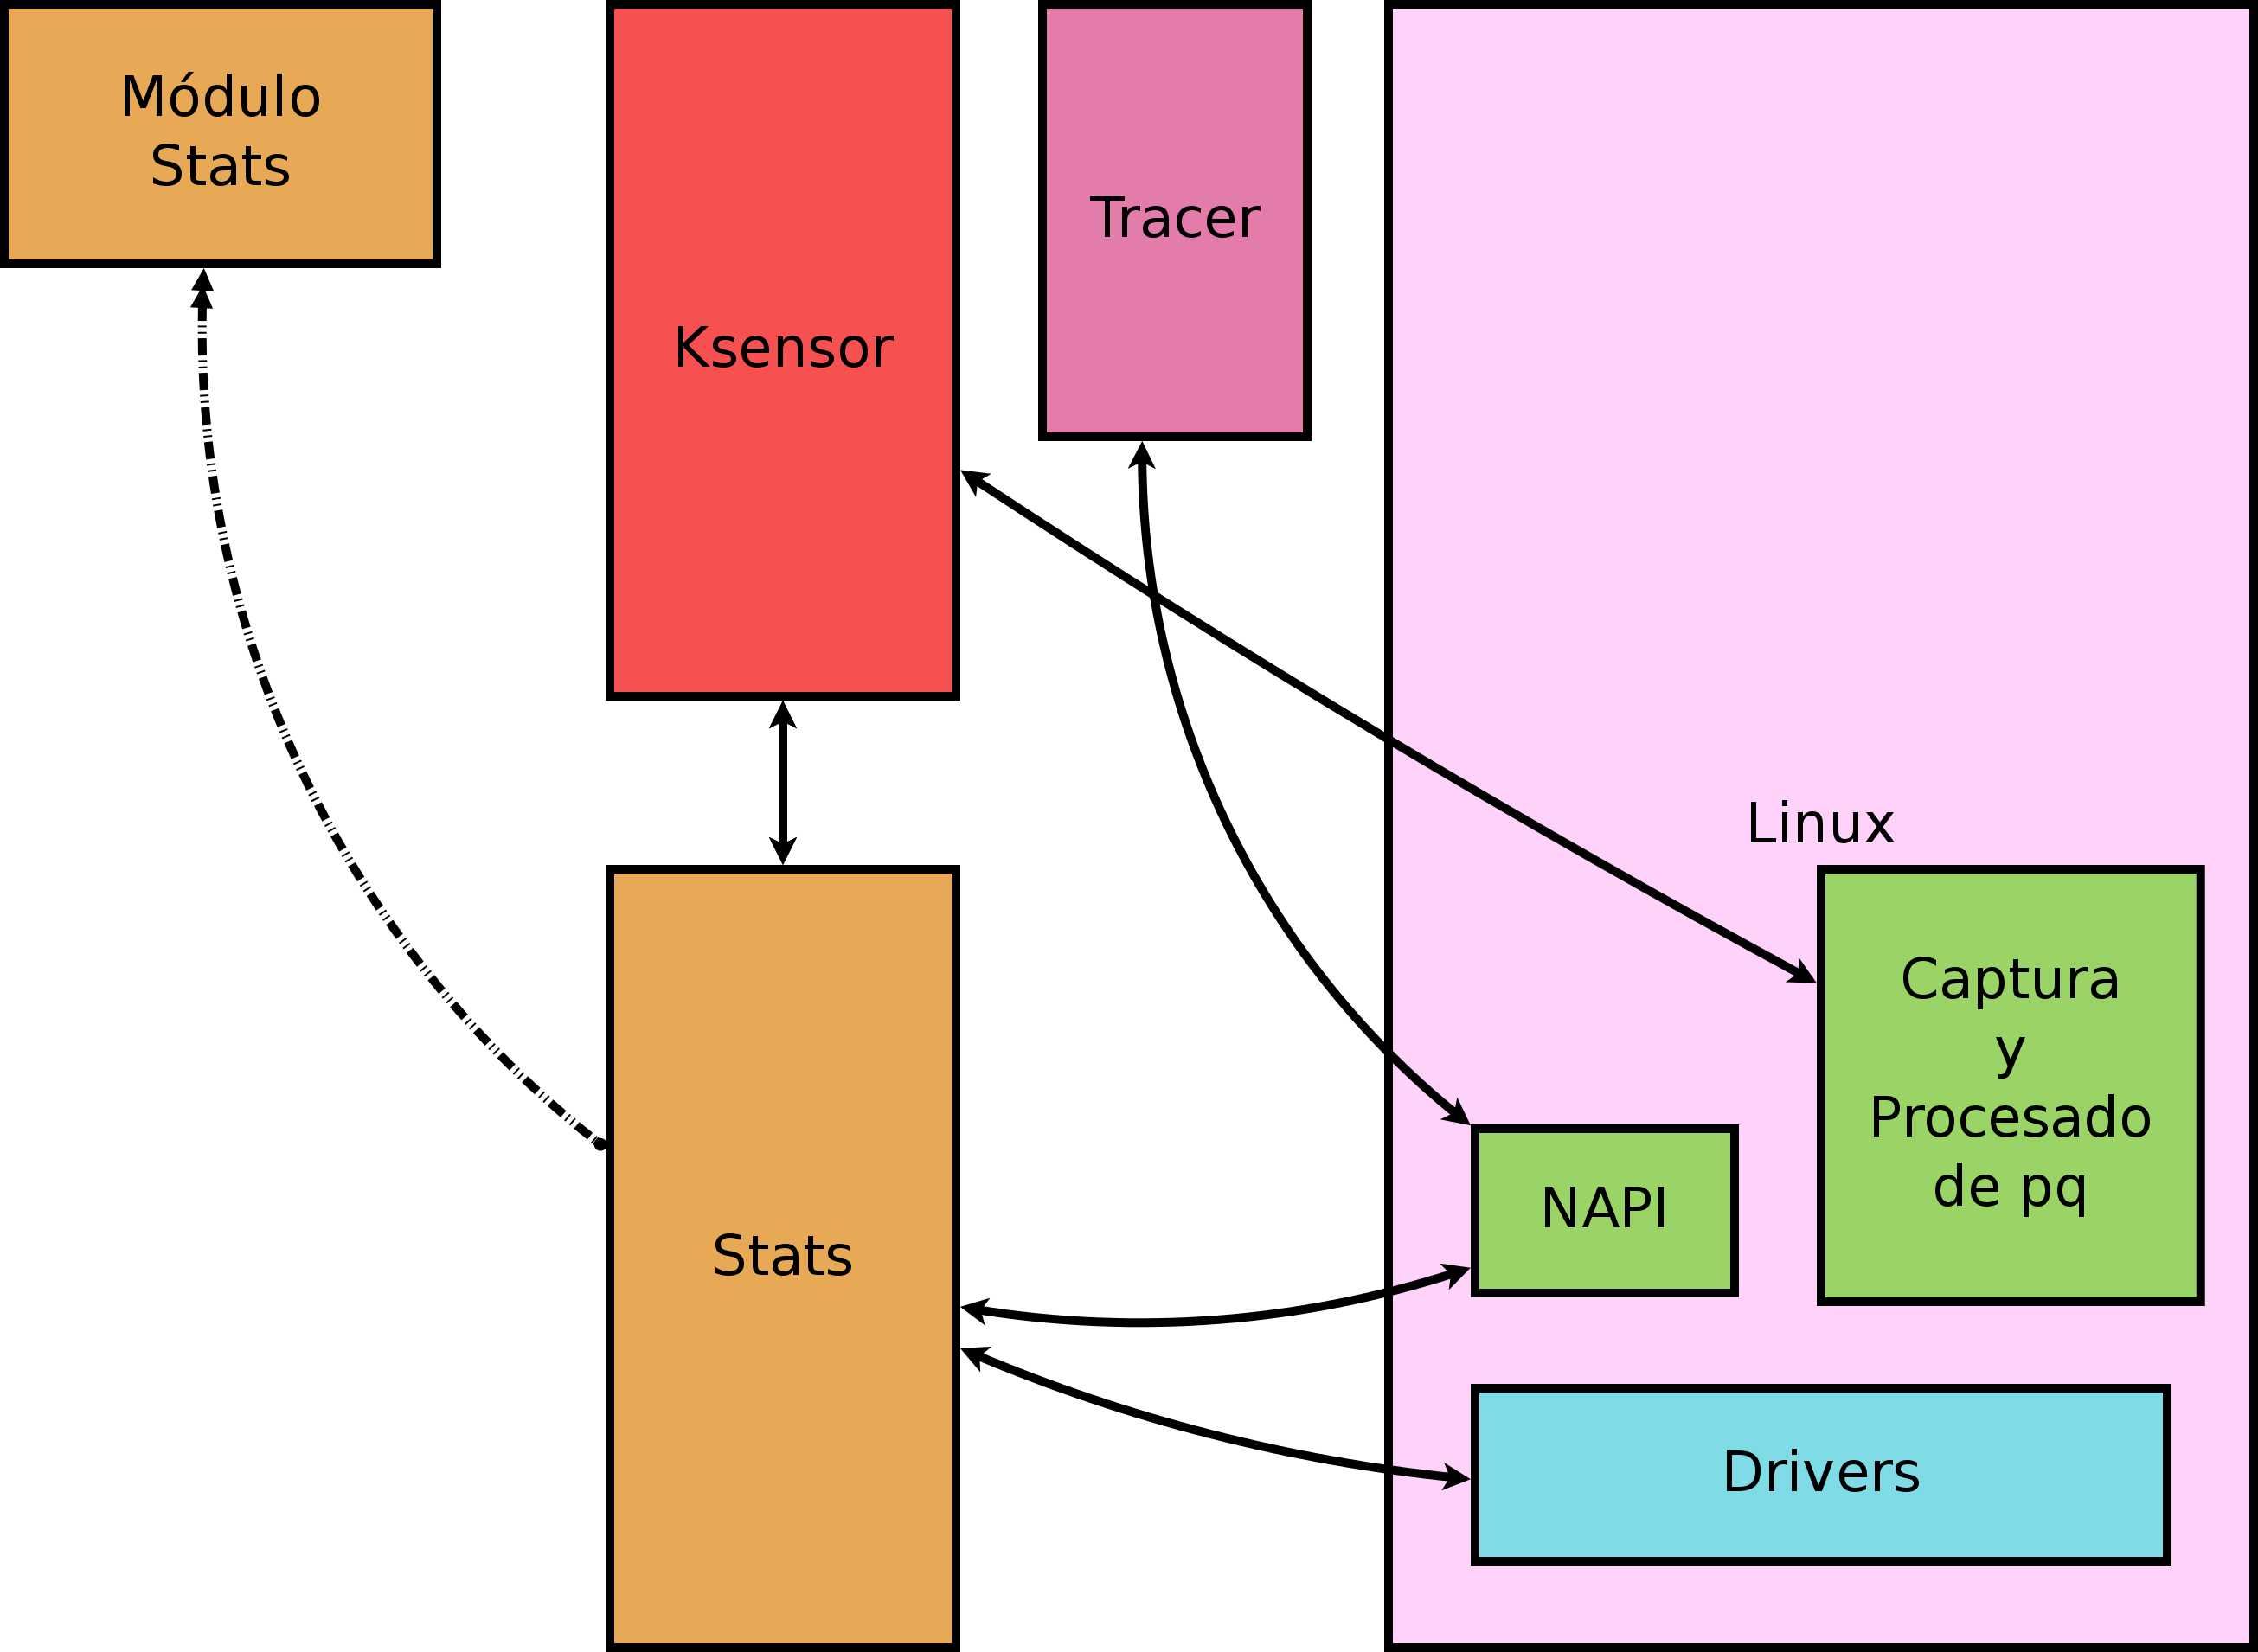
\includegraphics[width=\linewidth]{Integracion}
\caption{Integraci�n de los m�dulos entre si}
\label{fig:integracion-modular}
\end{figure}

En la figura, se han referenciado las 3 partes que componen el kernel, y donde se introduce o modifica c�digo. Apoyando la explicaci�n en la figura, se explicar� la integraci�n entre ksensor y los m�dulos.

\section{Ksensor y el m�dulo de estad�sticas}

En la figura se ha representado el m�dulo de estad�sticas como un m�dulo compuesto de dos partes, una propiamente dicha, el m�dulo, la parte que se puede insertar y extraer, y la parte que est� est�ticamente integrada en el kernel.

Dependiendo de las opciones de compilaci�n, en caso de habilitar Ksensor y el m�dulo de estad�sticas simult�neamente, se activan directamente las estad�sticas dentro de Ksensor, a parte de las estad�sticas internas del mismo. En caso de no habilitar Ksensor, el m�dulo de estad�sticas se compilar�a con solo una parte de las mismas.

\section{Ksensor y el m�dulo de trazas}

Este m�dulo ha sido dise�ado para tener un funcionamiento al margen de Ksensor, y de hecho en la implementaci�n actual, tracea softirqs, por lo que no se perder�a funcionalidad en este. En caso de implementar trazas dentro de Ksensor, se dejar�an de compilar, pero este m�dulo quedar�a disponible para el resto del sistema.

\section{Estad�sticas y trazas}

Entre estos dos m�dulos, al requerir en algunas partes de c�digo efectuar las mismas medidas, solo interact�an a nivel de implementaci�n. En el dise�o de bajo nivel se dar�n explicar� de una forma m�s concreta el tipo de interacci�n que tienen.
\chapter{Entorno de pruebas}

En este cap�tulo, se describir�n los dos programas que permiten al entorno de pruebas utilizar los m�dulos desarrollados en este proyecto, el m�dulo de estad�sticas y el m�dulo de traceo.

Se explicar�n en secciones separadas y se desarrollar� la l�gica que se ha seguido para su integraci�n con el agente de la sonda.

\pagenumbering{Roman}

\bibliography{../bibliography}

\printindex

\end{document}
